\documentclass[12pt,fleqn]{article}\usepackage{../../common}
\begin{document}
Uygulama - Yağmur Yağış Verisi


\begin{minted}[fontsize=\footnotesize]{python}
import pandas as pd
df = pd.read_csv('rainfall.csv',index_col=0,parse_dates=['dt'])
x = df[df.index.month == 3]['Daily Rainfall Total (mm)']
\end{minted}

\begin{minted}[fontsize=\footnotesize]{python}
from scipy.stats import gamma
res = gamma.fit(df['Daily Rainfall Total (mm)'])
a,loc,scale = res  
x.hist(density=True)
plt.ylim(0,0.4)
plt.plot(x, gamma.pdf(x,a,loc,scale),'r.')
plt.savefig('stat_176_app1_01.png')
\end{minted}

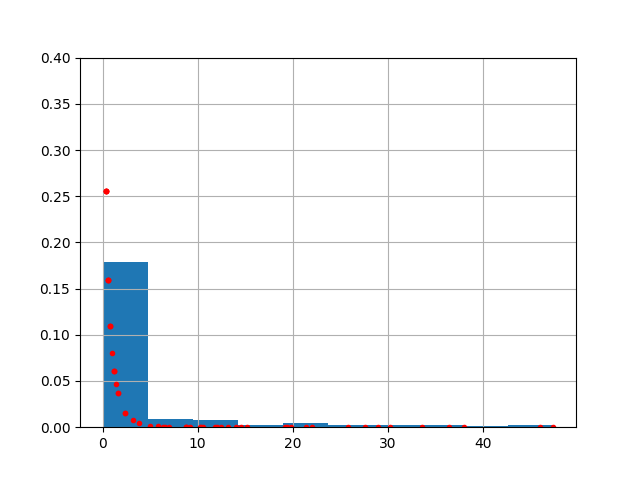
\includegraphics[width=20em]{stat_176_app1_01.png}

\begin{minted}[fontsize=\footnotesize]{python}
from scipy.stats import weibull_min
res = weibull_min.fit(df['Daily Rainfall Total (mm)'])
a,loc,scale = res  
x.hist(density=True)
plt.ylim(0,0.4)
plt.plot(x, weibull_min.pdf(x,a,loc,scale),'r.')
plt.savefig('stat_176_app1_02.png')
\end{minted}

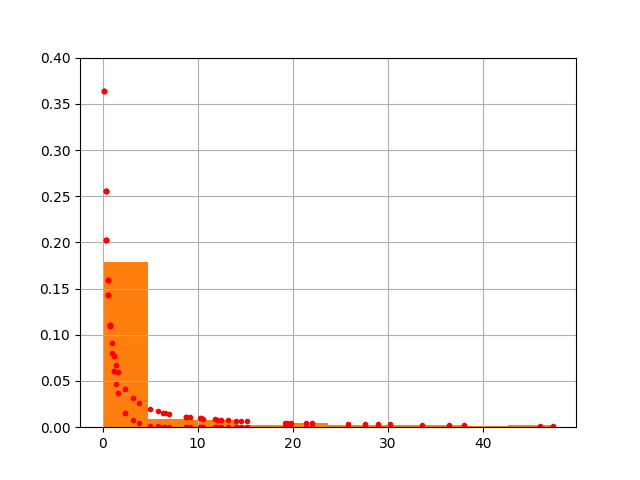
\includegraphics[width=20em]{stat_176_app1_02.png}

















\end{document}
